\documentclass[review]{elsarticle}

\usepackage{lineno,hyperref}
\modulolinenumbers[5]
\usepackage[margin=2cm]{geometry}
\usepackage{amsmath}
\usepackage{subcaption}
\usepackage{graphicx}
\usepackage[justification=centering]{caption}
\usepackage{tikz}
\usepackage{multirow}
\journal{Ecological Informatics}

%%
%% Guide for authors : https://www.elsevier.com/journals/ecological-informatics/1574-9541/guide-for-authors
%%
%%
%% Editor Latex instructions : https://www.elsevier.com/authors/author-schemas/latex-instructions
%%



%%%%%%%%%%%%%%%%%%%%%%%
%% Elsevier bibliography styles
%%%%%%%%%%%%%%%%%%%%%%%
%% To change the style, put a % in front of the second line of the current style and
%% remove the % from the second line of the style you would like to use.
%%%%%%%%%%%%%%%%%%%%%%%

%% Numbered
%\bibliographystyle{model1-num-names}

%% Numbered without titles
%\bibliographystyle{model1a-num-names}

%% Harvard
%\bibliographystyle{model2-names.bst}\biboptions{authoryear}

%% Vancouver numbered
%\usepackage{numcompress}\bibliographystyle{model3-num-names}

%% Vancouver name/year
%\usepackage{numcompress}\bibliographystyle{model4-names}\biboptions{authoryear}

%% APA style
%\bibliographystyle{model5-names}\biboptions{authoryear}

%% AMA style
%\usepackage{numcompress}\bibliographystyle{model6-num-names}

%% `Elsevier LaTeX' style
\bibliographystyle{elsarticle-num}
%%%%%%%%%%%%%%%%%%%%%%%

\begin{document}

\begin{frontmatter}

  \title{Automated Morphometrics using Deep Neural Networks : Case Study on a Beneficial Insect Species}

%\tnotetext[mytitlenote]{Fully documented templates are available in the elsarticle package on \href{http://www.ctan.org/tex-archive/macros/latex/contrib/elsarticle}{CTAN}.}



%% Group authors per affiliation:
\author[labri,itdlu]{Le Van Linh\corref{cor1}}
\ead{van-linh.le@labri.fr}
\author[labri]{Zemmari Akka}
\author[igepp]{Marie Alexia (?)}
\author[labri]{Beurton-Aimar Marie\fnref{ba}}
\author[igepp]{Parisey Nicolas\fnref{ba}}

\fntext[ba]{both authors contributed equally to this work.}
\cortext[cor1]{Corresponding author} 

%% %% or include affiliations in footnotes:
\address[igepp]{UMR 1349 IGEPP, BP 35327, 35653 Le Rheu, France}
%% \ead[url]{www.elsevier.com}

\address[labri]{University of Bordeaux, 351, cours de la Libération, 33405 Talence}
\address[itdlu]{Dalat University, Dalat, Lamdong, Vietnam}
%% \cortext[mycorrespondingauthor]{Corresponding author}
%% \ead{support@elsevier.com}

%% \address[mymainaddress]{1600 John F Kennedy Boulevard, Philadelphia}
%% \address[mysecondaryaddress]{360 Park Avenue South, New York}

\begin{abstract}
\textit{Aims:} \ldots \textit{Methods:} \ldots \textit{Conclusions:} \ldots
Landmark is one of the important concepts in morphometry analysis. Finding landmarks is not only used to measure the shape of the object but also applied to analyze the inter-organisms variations. Currently, the landmarks are mostly determined manually by the biologist.
In this work, we propose a method to automatic predict the landmarks on biological images: Deep Learning, more specific is Convolutional Neural Network (CNN). We proposed a CNN architecture which was built from the ``elementary blocks". Each block is made up of some popular layers of CNN.
The network then trained and tested on a dataset includes five parts of beetle (head, elytra, pronotum, left and right mandibles).
These works have also introduced another procedure to augment the dataset which can see a little bit small in our case.
In the experiments, we apply two strategies to evaluate the network and to improve the obtained results: training from scratch and applying a fine-tuning step.
The predicted landmarks from the network have been compared with the manual landmarks which provided by the biologists. The obtained results have proved that the predicted landmarks are considered to be statistically good enough to replace the manual landmarks.
\end{abstract}

\begin{keyword}
Landmarks \sep morphometry \sep deep learning \sep CNN
\end{keyword}

\end{frontmatter}

\linenumbers

\section{Introduction}

In the context of ecosystem services, there is an interest in studying complex interactions between evolution of insect populations and environmental factors affecting their functions. In order to assess specifically pest-regulating services and in line with studies pointing to shape traducing function \cite{klingenberg_evolution_2010}, there are more and more research about beneficial insect morphometrics \cite{sasakawa_utility_2016,raymond_combination_2014}. 
 In such morphometric studies, it is common to analyze subject's shape independently of their poses and sizes \cite{kendall_diffusion_1977}. Since the late $20^{th}$ century \cite{bookstein_foundations_1982}, rooted in a strong statistical background, geometric morphometrics addresses the study of such biological shapes \cite{rohlf_applications_1998}. It is an effective set of methods with several specialised softwares readily available \cite{adams_geomorph:_2013,klingenberg_morphoj:_2011}. Classical geometric morphometrics uses a set of landmarks to describe shape, a landmark being a two-dimensional anatomically-relevant point. In order to investigate the possibility of automated morphometric geometrics on beneficial insects, we chose to focus on one of the most common and ubiquitous beneficial insect of north-western France, \textit{Poecilus cupreus} (Carabidae). It is considered a polyphagous predator \cite{larochelle_1990} beneficial to agriculture, being able to consume a large variety of agricultural pests including weed seeds, slugs and aphids \cite{kromp_carabid_1999}. As a Coleoptera, its morphological variability is usually measured on exoskeleton structures such as the head, pronotum and elytra \cite{eldred_does_2016}. \\
 
Of course, the first step in any morphometric geometrics study is the digital imaging of the biological specimens, usually with controlled illumination and contrasting background. As such, morphometric landmark detection and positioning can be though as a particular problem of features detection and solved using robust digital image processing \cite{gonzalez_digital_2006}. In the recent years, the term ``deep learning" emerged describing class of computational models composed of multiple processing layers learning representations of data with multiple levels of abstraction \cite{lecun2015deep}. Each layer extracts the representation of the input data from the previous layer and computes a new representation for the next layer. In the hierarchy of model, higher layers of representation enlarge aspects of the input that is important for the computational task (classification, regression, \ldots) and suppress irrelevant variations. As supervised learning algorithms, they use gradient descent optimization method to update the learnable parameters via backpropagation. Deep learning algorithms have proved to be very efficient in a wide variety of domains, notably image recognition and classification \cite{krizhevsky2012imagenet,ciregan2012multi,szegedy2015going}, speech recognition \cite{mikolov2011strategies, hinton2012deep, sainath2013deep}, question answering \cite{bordes2014question} and language translation \cite{sutskever2014sequence, jean2014using}.
Within deep learning, Convolutional Neural Networks (CNNs) are well known for their success in many computer vision tasks such as image classification \cite{krizhevsky2012imagenet,ciregan2012multi} and  objets recognition \cite{li2015convolutional,tompson2014joint}.
Recent success of this algorithm in human biometry \cite{cintas2016automatic} lead us to believe in its potential for insect morphometrics.  

\subsection{Related works}\label{rw}

Landmark or point of interest is a specific point that may contain the useful information. For example, the tip of the nose or the corners of the mouth are landmarks on human face. In image processing, we can consider two kinds of cases: the object of interest can or not be segmented. Setting landmarks can not be achieved in the same way depending on which situation we are. When segmentation can be applied, Lowe et al. \cite{lowe2004distinctive} have proposed SIFT method to find the corresponding keypoints between two images. Palaniswamy et al. \cite{palaniswamy2010automatic} have proposed a method based on probabilistic Hough Transform to automatically locate the landmarks in digital images of Drosophila wings. In our work \cite{le2017maelab}, we have proposed a method which have been extended from Palaniswamy's method, to determine landmarks on mandibles of beetles. The mandibles of beetle have the simple shape and easy to segment. We have obtained good enough results about determining the landmarks automatically on mandibles. Unfortunately, this method can not be applied to other parts of beetles than the pronotum seems is segmentation has too many noises.

In recent years, deep learning is known as a solution in computer vision. Using convolutional network to determine the landmarks on 2D images has achieved better results and it seems that good solutions for the images that can not segment. Yi Sun et al. \cite{sun2013deep} have proposed cascaded convolutional neural networks to predict the facial points of interest on the human face.
Zhanpeng Zhang et al. \cite{zhang2014facial} proposed a \textit{Tasks-Constrained Deep Convolutional Network} to optimize facial landmarks detection. The model determines the facial landmarks with a set of related tasks such as head pose estimation, gender classification, age estimation, face recognition, or facial attribute inference. In biology field, Cintas et al. \cite{cintas2016automatic} has introduced a network to predict the landmarks on human ears. After training, the network has the ability to predict 45 landmarks on human ears. In this way, we have applied CNN computing to work with pronotum landmarks.

\subsection{Contributions}

We present an approach to predict morphometric landmarks based on standardized digital pictures of a coleoptera anatomical parts. For each anatomical parts, we train a convolutional neural network and statisticaly assess the suitability of the predicted landmarks to replace manual landmarks in further geometric morphometric studies.

\section{Material and Methods}

In the context of this section, we first present the dataset that we have used in this study, as well as the strategies to pre-process the data. Then, we show the network architecture model that we have designed to predict the landmarks in the beetle's images.

\subsection{Dataset and preprocessing}
In order to provide the experiment data, we have selected the Brittany lands (North-West of France) to collect the samples. After collecting in three months, a collection of $293$ beetles has been established ($147$ males and $146$ females/ $155$ organic and $138$ conventional) (Figure \ref{imgbeetle}). As usual, images of beetles have been chosen to be studied instead of using real objects for pratical reasons. The pictures of each body parts were captured under a trinocular magnifier at $\approx 300$ pixels/mm for elytra, $\approx 600$ pixels/mm for pronotum and head, $1500$ pixels/mm for mandibles. One can note that the head, pronotum, and elytra parts have been captured before dissection. The left and right mandibles have been separated from the beetle's body before taking the photos. All the images have been taken with the same camera under same conditions to release in the RGB color mode with the size of $3264 \times 2448$.

\begin{figure}[h!]
	\centering
	\begin{tikzpicture}
		\node (img1) {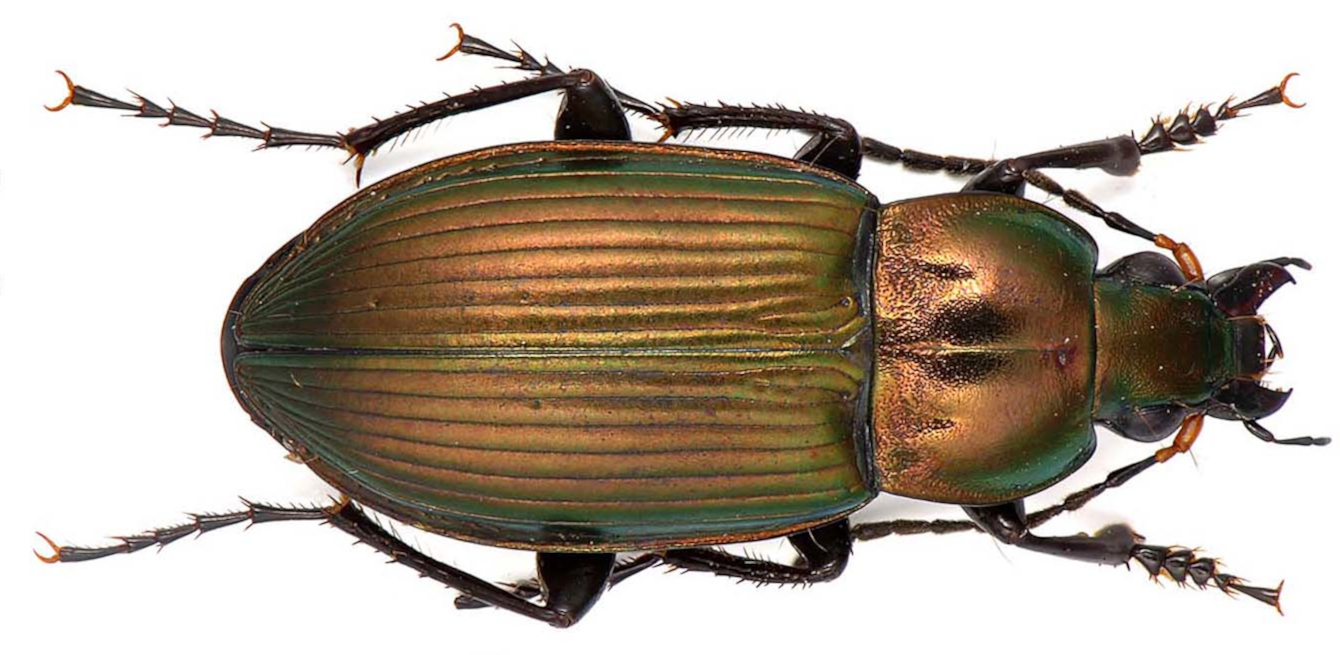
\includegraphics[width=0.60\textwidth]{images/beetle2}};
		\draw[thick,<->] (-3.2,-2.5) -- (4.7,-2.5);
		\node at (1, -2.7) {\footnotesize{12 mm}};	
	\end{tikzpicture}
	\caption{An illustration of the beetle.}
	\label{imgbeetle}
\end{figure}

In the next step, morphological landmarks were first set manually on the dorsal views of each body part of the beetles (head, pronotum, elytra, right and left mandibles). The morphology of each body part was processed and analyzed separately in order to limit variation resulting from their relative positions due to articulation. Landmarks were chosen according to the ease and the precision of their location on each specimen (Figure \ref{figdatasamples}). Replicability analyses were performed to confirm the accuracy of landmarks positioning. They were positioned on each picture with TPSDig2 software (version 2.17) (Rohlf, 2013a). In some individuals, mandibles could not be processed because they were lacking or broken. For each specific part, a set of number of landmarks has been provided, for example, \textit{$8$ landmarks for pronotum, $10$ landmarks for head, $11$ landmarks for elytra, $16$ and $18$ landmarks for left and right mandibles, respectively} (Figure \ref{figdatasamples}). In the context of this study, these manual landmarks have been used as ground truth to evaluate the output of our method.

\begin{figure}[h!]
    \centering
    \subcaptionbox{. Pronotum.}{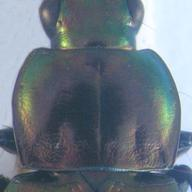
\includegraphics[width=0.19\textwidth]{./images/Prono_010}}~~
\subcaptionbox{. Head.}{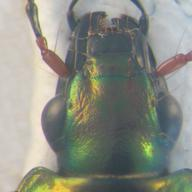
\includegraphics[width=0.19\textwidth]{./images/Tete_009}}~~
\subcaptionbox{. Elytra.}{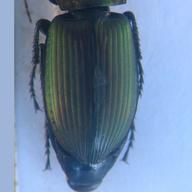
\includegraphics[width=0.19\textwidth]{./images/Elytre119}}~~
\subcaptionbox{. Left mandible.}{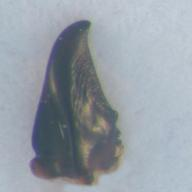
\includegraphics[width=0.19\textwidth]{./images/Mg_021}}~~
\subcaptionbox{. Right mandible.}{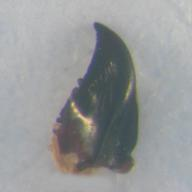
\includegraphics[width=0.19\textwidth]{./images/Md_015}}~\\
	\subcaptionbox{. Pronotum.}{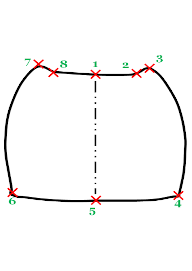
\includegraphics[width=0.19\textwidth]{./images/pronotum_mlm}}~~
\subcaptionbox{. Head.}{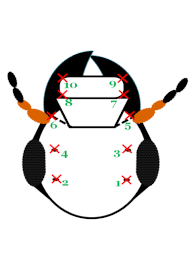
\includegraphics[width=0.19\textwidth]{./images/tete_mlm}}~~
\subcaptionbox{. Elytra.}{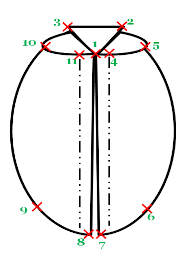
\includegraphics[width=0.19\textwidth]{./images/elytre_mlm}}~~
\subcaptionbox{. Left mandible.}{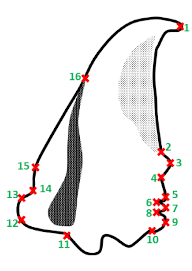
\includegraphics[width=0.19\textwidth]{./images/lmandible_mlm}}~~
\subcaptionbox{. Right mandible.}{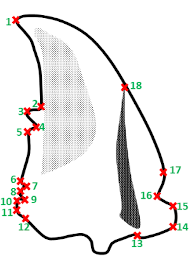
\includegraphics[width=0.19\textwidth]{./images/rmandible_mlm}}~\\
    \caption{The sample images in our dataset (top row) and manual landmarks on each part defined by biologists (bottom row).}
    \label{figdatasamples}
\end{figure}

The success stories \cite{} have proved that CNN models have been trained on a large dataset with an enormous number of data samples before using it to perform on testing data. Training the model with a big dataset can help the model able to learn more different cases and to improve the learning ability of the network. Unfortunately, providing a large dataset is too costly in several domains, e.g., in biology, medical. A solution to deal with this problem is to create the misshapen data from real data and to add them to the dataset. In our case, we have only 293 images for each part of the beetles. This number is large from the point of view of manual operations, but it is not enough to apply deep learning methods. So, we have augmented the number of images in each set of images.

Most often in deep learning applications, dataset augmentation uses operations such as translation, rotation, or scaling, which are well-known efficient to generate the new version of existing images \cite{}. However, these operations can be invariant in some cases \cite{}. We have done some tests by moving the object in the picture. In each time, we have quickly gone to the over-fitting in the training step (more detail in Section X). Consequently, we have preferred different ways to produce misshapen images by operating on the image's color channels. We have proposed two strategies to augment the number of images in our dataset.

The first strategy was applied to change the value of each channel in the original image. According to this, a constant have been added to a channel of RGB image for each time. For example, if we add a constant $c = 10$ to the red channel from an original RGB image, we will obtain a new image with the values at red channel by greater than the red channel of original image a value of $10$. By this way, we can generate three new RGB images from a RGB image.

The second procedure was split the channels of RGB images to create three gray-scale images. This work seems promising because the network model on single-channel images. At the end, we have generated six versions from an image. In total, we have obtained $293 \times 7 = 2051$ images for each set of images. Figure \ref{figdataauge} illustrates the two strategies that we have described.

\begin{figure}[h!]
    \centering
    \subcaptionbox{. Add a constant to each channel.}{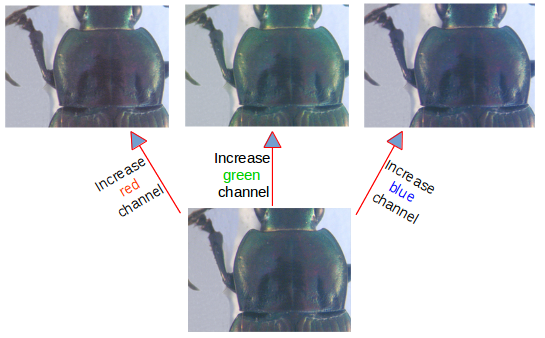
\includegraphics[width=0.49\textwidth]{./images/inc_channels}}~~
\subcaptionbox{. Split the channels of image.}{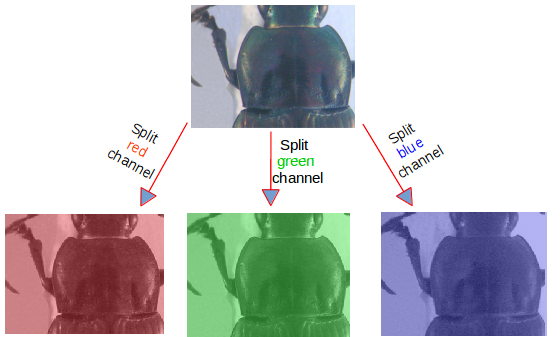
\includegraphics[width=0.49\textwidth]{./images/sp_channels}}
    \caption{The two strategies to augment the number of images in our dataset.}
    \label{figdataauge}
\end{figure}

To perform the objective, we have observed the input size of the several CNN models and noticed that their input sizes were limited to $256$ pixels. One can note that our images were released with the size of $3264 \times 2448$, as mentioned in Section \ref{}. This size has a bit heavy for training the network. Consequently, we have down-sampled our images to a new size of $256 \times 192$ to respect the ratio between width and height. Of course, coordinates of landmarks have been down-sampled to the new size of images. Practically, convergence is usually faster if the average of each input variable over the training set is close to zero. According to \cite{lecun2012efficient}, the brightness of the image is normalized to $[0,1]$, instead of $[0,255]$ and the coordinates of the landmarks are normalized to $[-1,1]$, instead of $[0,256]$ and $[0,192]$ before giving to the network.

\subsection{Network architecture}
From the first appearance to current, many CNN architectures have been available. Most often, they were designed to solve specific problems. 

The first model has been inspired by AlexNet architecture. It received gray-scale image with the size of $256 \times 192$ as the input. The image is analyzed by three repeated structures of a convolution (CONV) layer followed by a maximum pooling (POOL) layer. As usual, the depth of CONV layers are set to increase from the beginning to the end with a small kernel. In our model, we have chosen $32, 64, 128 $ for the depths and $ 3 \times 3, 2 \times 2, 2 \times 2 $ for the kernel'sizes of CONV layers, respectively. Using POOL layers after the CONV layers is a common occurrence in CNN \cite{}. This work towards to two advantages: reducing the spatial size of the representation to decrease the number of parameters as well as saving the computing time, and to prevent the over-fitting during the training process. In the first model, we have used the common form for a POOL layer: a filter with the size of $2 \times 2$ and a stride of $2$ pixels. With these parameter values, the spatial size of the image will be halved after every POOL layer. In order to extract the global relationship between the features and to provide the prediction, three fully-connected (FC) layers have been added after the combination of CONV-POOL. The first FC layer takes all features from the last POOL layer as the input for computing. Then, the computed results will be passed through the activation functions to provide the outputs. The second FC layer receives the outputs of the first FC layer as the input. The process at this layer is the same than the first one. The third FC layer accepts the outputs of the second FC layer, then they will be used to compute the input. It is worth to note that we keep the linear value for the output of the third FC layer. The number of outputs at each FC layers is set to $500, 500$, and $X$, respectively. The number $X$ equals to two times the number of landmarks that we want to predict, for example, to predict $8$ landmarks on pronotum, we have set $16$ as the outputs of the last FC layer. The first model has been trained and tested on our pronotum images. Nevertheless, the obtained results have not been considered good enough to use it. The main problem comes from the appearance of over-fitting during the training process. The detail of this experiment will be discussed in Section X.

As an attempt to remove over-fitting, we have increased the number outputs of the first two FC layers from $500$ to $1000$ with a hypothesis considering more features. However, the obtained results have not changed, the over-fitting was not suppressed.

In order to build the third model, we have defined a concept of Elementary Block (EB). Figure \ref{figeblock} illustrates the order of the classes in an EB, it is defined as a sequence of a CONV layer, a maximum POOL layer, and a Dropout layer. As usual, the dropout layers are inserted between the FC layers to prevent the over-fitting as we have seen in the success stories \cite{}, but we have added them in the extracting features blocks to create some kinds of image noise augmentation. The objective of this work is to provide more studied cased in each training iteration. Besides, dropout layer will randomly drop some connections during the training process. It makes the network thinner than the original one (less parameters), and training a network with dropout layer is equalivalent to train a set of thinner networks. These works have significantly reduced over-fitting and given more major improvements than other regularization methods \cite{}.

\begin{figure}[h!]
	\centering
	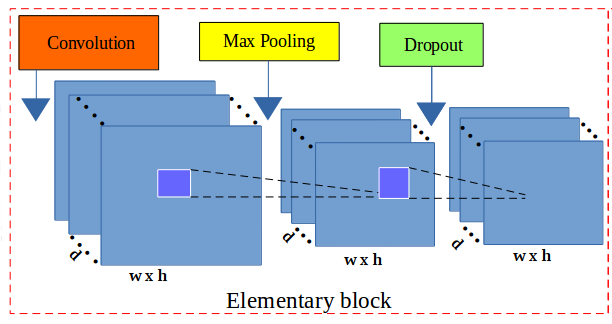
\includegraphics[width=0.6\textwidth]{images/elementary_block}
	\caption{The components of an elementary block}
	\label{figeblock}
\end{figure}

For our critical objective, we have initially assembled three Elementary Blocks to create the third model, so-called Elementary Blocks Network (EB-Net). The used parameters of the convolution and the pooling layers have been kept in the same configuration as the second model. The probabilities of the dropout layers, which were added after the pooling layers, are set increasing: $0.1, 0.2$, and $0.3$, respectively. Following the three EBs is three fully-connected layers with a similar number of outputs as the second model. Moreover, a dropout layer with the probability equals to $0.5$ has been inserted between the first and the second fully-connected layers. Figure \cite{figebnet} shows the structure of the EB-Net.

\begin{figure}[h!]
	\centering
	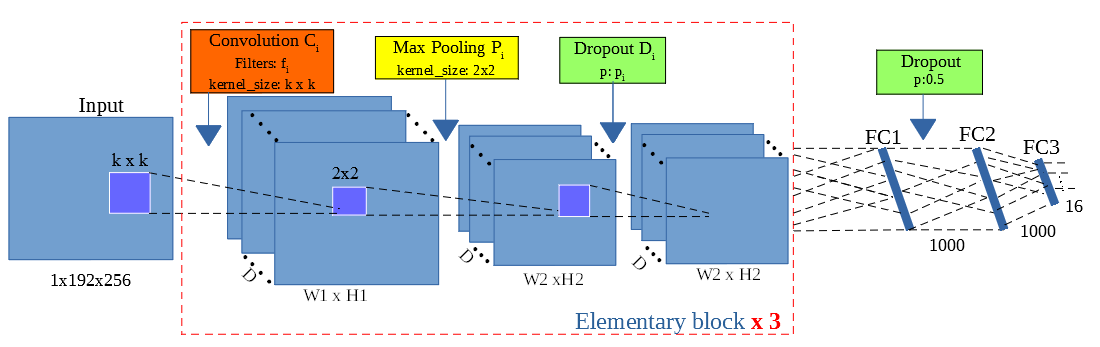
\includegraphics[width=0.8\textwidth]{images/model3}
	\caption{Elementary Blocks Network (EB-Net) architecture}
	\label{figebnet}
\end{figure}

In a CNN model, besides the model-specific hyper-parameters which involve the structure of the network (e.g., the number of layers or parameter values for each layer), the optimized hyper-parameters are also important variables in designing a CNN model. These variables are related to train a network model, for example, the loss function, number of epochs, or initialized values of learning rate, batch size. Practically, these values depend on the task and the dataset, they are determined empirically. In our application, we have chosen gradient descent as the optimized algorithm as usual studies \cite{}. Consequently, the learning rate begins from $0.03$ and to stop at $0.00001$; whereas the momentum rate is updated from $0.9$ to $0.9999$. During the training, the learning and momentum rates are adjusted to fit with the number of epochs. Besides, the Root Mean Square Error (RMSE) has been chosen to use as the loss function because it is usually used for regression problems where outputs are not discrete values as in the case of landmark coordinates. 

\subsection{Setting and training EB-Net}
In order to provide the predicted landmarks for all images, we have applied cross-validation technique to select the test images, we will call a selection step is a round. For each round, we take $33$ images and keep them for testing. The $260$ remaining images will be used to train and to validate the network model. It is worth to note that the set of $260$ images has been augmented by the strategies described in Section Y, to provide $1820$ images for these two steps. To achieve the cross-validation steps, we have to do $9$ rounds in total. 

During the training and validation step, $1820$ images are randomly divided into two sets with a ratio of $60\% : 40\%$ and used for the corresponding processes (training : validation). In each training step, the pair of \textit{image} and \textit{its manual landmarks} is inputted to train the network model. In our cases, the manual landmarks have been given by the biologists. So, they can be used as ground truth to train the network, as well as to evaluate the predicted ones. The EB-Net has been implemented by using Lasagne framework \cite{}, and trained in $5000$ epochs on Linux system by using a NVIDIA GPU (Titan X) card.

\section{Results}
\subsection{The first test}
As mentioned in Section X, we have three models for predicting landmarks. In order to select the best one for our objective, we have first tested the three models on pronotum, before applying the best one on the two other parts of beetle (head and elytra).

\begin{figure}[h!]
    \centering
    \subcaptionbox{. Losses of the first model.}{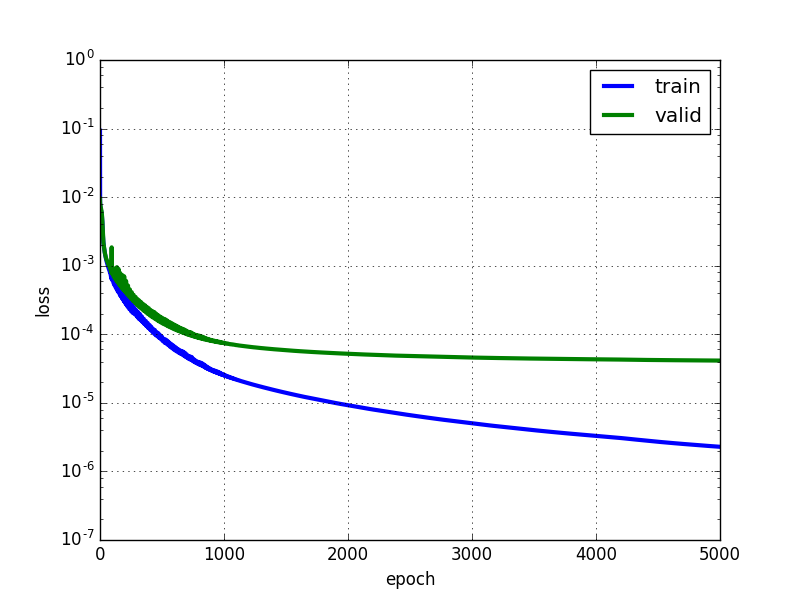
\includegraphics[width=0.49\textwidth]{./images/loss_model_1}}~~
\subcaptionbox{. Losses of EB-Net.}{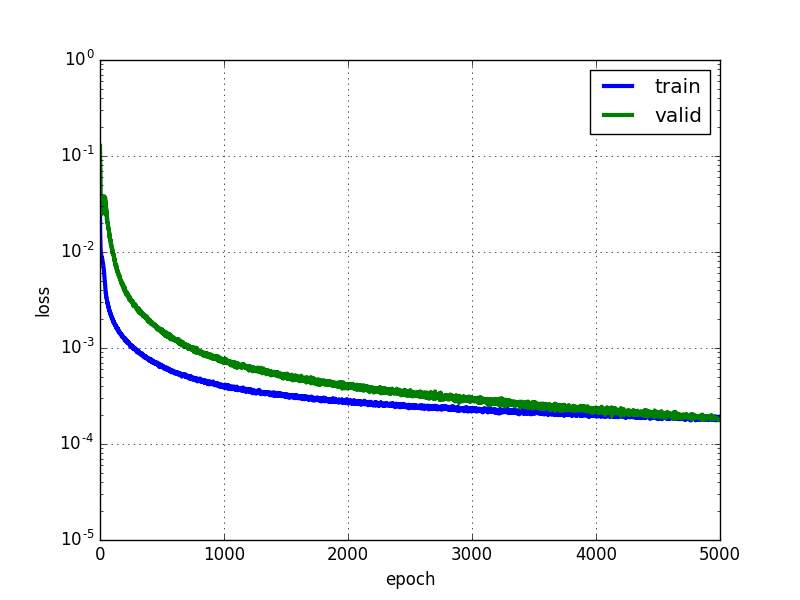
\includegraphics[width=0.49\textwidth]{./images/loss_v16}}
    \caption{The losses of two models on pronotum images.}
    \label{figdlosses}
\end{figure}

Figure \ref{figdlosses} shows the losses during the training and validation processes of two models (the first one and EB-Net) on pronotum images. The blue curves are training losses, and the green curves are validation losses. In the first model (Figure \ref{figdlosses}a), the training loss ables to decrease along with the number of epochs, but the validation loss is stable after $2000$ epochs. Clearly, the over-fitting has appeared in the fist model. In the second model, no concrete change appears in the curves even the parameters of fully-connected layers have been modified. We have also checked the losses of the second model, the result is also the same as the first one. So, we have not mentioned it in this document. On the opposite side of the first two models, the losses of EB-Net (Figure \ref{figdlosses}b) is really different. They are far from the beginning, but become more close at the end of process. One can note that the over-fitting has disappeared in this architecture. Therefore, we can assume that using elementary block works well to prevent over-fitting in our case. For these reasons, we have decided to use EB-Net for producing the landmarks.

In order to achieve the best quality of predicted landmarks, we have tested EB-Net in two different strategies: training from scratch and transfer learning. The following sections describe detailed results from these processes. Firstly, we consider the losses during the training and validation processes. Secondly, we compare the coordinates of predicted landmarks and corresponding manual ones by calculating the distance between them. The average distance is also taken into account for each landmark position. We display also the landmarks on the image. Finally, the distribution of distances will be discussed in some cases of landmarks. 

\subsection{Training from scratch}
In the first strategy, EB-Net has been separately trained on three sets of images: pronotum, head, and elytra. Table \ref{tbltrainingloss} shows the losses of 9 rounds when we train EB-Net on pronotum images. We can observe the losses are tiny in each round, and the differences among rounds are not various even we have altered images in each step.

\begin{table}[h!]
	\centering
	\begin{tabular}{l l l}
	Round & Training loss & Validation loss \\ \hline
	1 & 0.00018 & 0.00019  \\ \hline
	2 & 0.00019 & 0.00021 \\ \hline
	3 & 0.00019 & 0.00026 \\ \hline
	4 & 0.00021 & 0.00029 \\ \hline
	5 & 0.00021 & 0.00029 \\ \hline
	6 & 0.00019 & 0.00018 \\ \hline
	7 & 0.00018 & 0.00018 \\ \hline
	8 & 0.00018 & 0.00021 \\ \hline
	9 & 0.00020 & 0.00027 \\ \hline
	\end{tabular}
	\caption{The losses during the training of the third model on pronotum images}
	\label{tbltrainingloss}
\end{table}

In the next step, we focus on the location of predicted landmarks by comparing these with the ground truths. We have calculated the distances (in pixels) between the manual landmarks and corresponding predicted ones. Then, the average distance on each position has been considered. Table X shows the average distance on each position of all three parts: pronotum, head and elytra. With the image's size of $256 \times 192$, we can consider that an error around $1\%$ ($\approx 2$ pixels) coud be an acceptable error. Unfortunately, our results exhibit the average distance around $4$ pixels for the best cases, and more than $5$ pixels in the worst cases.

\begin{table}[h!]
	\centering	
	\begin{tabular}{|c|c|c|c|c|c|c|c|c|c|c|c|}
		\hline
		\textbf{LM} & 1 & 2 & 3 & 4 & 5 & 6 & 7 & 8 & 9 & 10 & 11 \\ \hline
		\textbf{Pronotum} & \textcolor{green}{4.00} & 4.48 & 4.3 & 4.39 & 4.29 & \textcolor{red}{5.36} & 4.64 & 4.94 & - & - & - \\ \hline
		\textbf{Head} & \textcolor{red}{5.53} & 5.16 & 5.38 & 5.03 & 4.84 & \textcolor{green}{4.45} & 4.79 & 4.53 & 5.14 & 5.06 & - \\ \hline
		\textbf{Elytra} & \textcolor{green}{3.87} & 3.97 & 3.92 & 3.87 & 4.02 & 4.84 & 5.21 & \textcolor{red}{5.47} & 5.27 & 4.07 & 3.99 \\ \hline
	\end{tabular}
	\caption{The average distances per landmark on images of each set.}
	\label{tblavgpronotum}
\end{table}

To illustrate the points, Figure \ref{figeb1} shows the predicted landmarks on the three parts of beetles. The red/yellow points present the predicted/manual landmarks. One can note that even some predicted landmarks are close to the manual ones, we have also some predicted coordinates that are far from the expected results.

\begin{figure}[h!]
	\centering
    \subcaptionbox{. Pronotum}{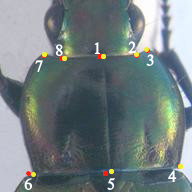
\includegraphics[width=0.31\textwidth]{images/Prono_001_2}}~~
	\subcaptionbox{. Head}{\includegraphics[width=0.31\textwidth]{images/Tete_006_2}}~~
	\subcaptionbox{. Elytra}{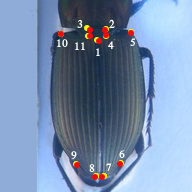
\includegraphics[width=0.31\textwidth]{images/Elytre007_2}}
    \caption{The landmarks on three parts of beetle. The red/ yellow points present the predicted/ manual landmarks.}
    \label{figeb1}
\end{figure}

It is worth to note that an average value could reflect two different cases: the values closed together (small dispersion) or two sets of values very far (large dispersion). In order to check the , Figure \ref{figprodist} shows the distribution of distances between the manual and predicted landmarks for the best and the worst cases in each set of images. Each point presents the distance between the points (landmarks) of an image. The lines illustrate the average distance in each case. In both of two cases (the best and the worst), the distances are most often stay in the region from 0 to the average value. However, it exhibits a small dispersion, some points are still far away the mean value.

\begin{figure}[h!]
    \centering
    \subcaptionbox{. The $1^{st}$ landmark \label{figc4lm1dist}}{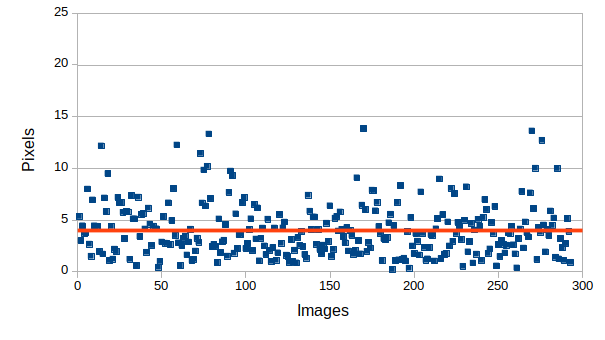
\includegraphics[width=0.48\textwidth]{./images/fs_lm1}}\hspace{0.5cm}
\subcaptionbox{. The $6^{th}$ landmark \label{figc4lm6dist}}{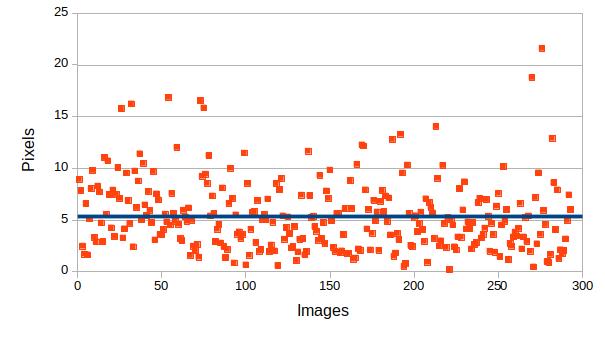
\includegraphics[width=0.48\textwidth]{./images/fs_lm6}}
    \caption{The distribution of distances between manual and corresponding landmarks of all pronotum images for the best ($1^{st}$ landmark) and the worst case ($6^{th}$ landmark)}
    \label{figprodist}
\end{figure}

The EB-Net has achieved good outcomes in most cases. However, it exists several difficult images in our dataset that the model can not recognize. That leads to the appearance of some high distance values in Figure X. The next step is to improve the predicted results.

\subsection{Transfer learning process}
Working with deep learning requires not only to design a good architecture but also to provide a large dataset to train and to test the model. Practically, this is a potential problem in some application domains as in biology. As mentioned in section X, we have augmented the number of images in our dataset and used it to train EB-Net. However, our number is far away several thousands images. In this case, knowledge transfer or transfer learning between tasks could be an advice. We describe this process in this section to improve our predictions.

Transfer learning \cite{} is a technique in deep learning to re-purpose a model, which has been designed for a specific task (called source task), on another related task (target task). Chosing which strategy of transfer learning to apply depending on the relationship between two tasks, as well as the size of database. Practically, transfer learning is mostly targeted on $2$ strategies:
\begin{itemize}
	\item \textbf{Use CNN as a fixed feature extractor}: Take a CNN pre-trained on a large dataset, then remove the last fully-connected and use the rest layers of CNN as a fixed extractor for the new dataset.
	\item \textbf{Fine-tuning a CNN}: This situation is the same as the first one. However, it does not only replace and retrain the last layer but also fine-tunes the weights of the pre-trained model by extending the backpropagation. One can note that to reuse a pre-trained model, the parameters have been adapted between two tasks. These parameters could be the size of input images, the number of outputs, or the parameters of each layer. As usual, the parameter values at each layer, e.g., padding or stride values, are selected to change their values to declare the differences between the two tasks.
\end{itemize}

As a preliminary work, we have tested several well-known models \cite{} that have been trained on ImageNet \cite{}. These pre-trained models have been shared in deep learning community as a source to re-use the features of ImageNet dataset. Unfortunately, the features from ImageNet seem that do not relevant for our application because Image features mainly concern the detection of global shape of the objects whereas landmarks can be considered as local features \cite{}. Luckily, searching for landmarks is well defined in other application such as face recognition, or facial keypoints detection. Consequently, we have decided to continue with EB-Net: we have pre-trained EB-Net with a public facial keypoints dataset, then transferred the pre-trained parameters to fine-tune on beetle's images.

\subsection{Pre-train EB-Net on facial keypoint dataset}

In recent years, several competitions have been published for predicting facial keypoints on human face, where they have publiced a dataset for training the models. As mention before, our problem has a revelant to these kind of competition. So, we have decided to choose a facial keypoints dataset to train EB-Net, and then to transfer the parameters to fine-tune on beetle's images.

The dataset that we have selected has been published for a challenge in the Kaggle website. It includes $2140$ images of human faces with a size of $96 \times 96$. Each image contains $15$ landmarks on the face: $6$ landmarks for eyes, $4$ landmarks for eyebrows, $4$ landmarks for the mouth, and $1$ landmark for nose tip. Figure X shows four face images in the dataset and the landmarks on each face.

In order to use EB-Net on this dataset, we have adapted the parameters of the input and the output layers to match with the requirements of the challenge. The new parameter values are $96 \times 96$ for the input size, and $30$ for the number of output (corresponding to $15$ landmarks). In hyper-parameters side, we have increased the number of epochs to $10000$ but kept the same for other values as training from scratch. As the first step, we take into account the RMSE score to evaluate and to compare the effectiveness of EB-Net with other published scores in the challenge.

\begin{table}[h!]
	\centering
	\begin{tabular}{ | c | c | c | c | c |}
	\hline
	\multirow{2}{*}{Team} & Olegra & Trump & Enes & \multirow{2}{*}{Our} \\
	  & $1^{st}$ & $2^{nd}$ & $3^{rd}$ &  \\ \hline
	RMSE score (in pixels) & 1.2824 & 1.4004 & 1.4026 & \textbf{1.497} \\ \hline
\end{tabular}	
	\caption{RMSE comparison between our score and top three of challenge.}
	\label{tblRMSE_challenge}
\end{table}

Table \ref{tblRMSE_challenge} shows the scores of top $3$ on the challenge board and our one. It is worth to note that their scores have been obtained by testing their models on a private set of images that we can not access. So, we have kept $100$ images in the public dataset for testing process. Comparing with these scores, the three models present better results than us but we are very close. In our opinion, the RMSE score around the 1 pixels is not so far if we would like to display the landmarks on the images. Consequently, we have the base to believe that EB-Net is still good in any way, and we have decided to re-use the pre-trained parameter values to fine-tune the model for beetle images. 

\subsection{Fine-tuning on beetle images}
As we have mentioned, fine-tuning is a strategy of transfer learning that we could boost the efficiency of a model on the target task. Technically, the weights of a CNN model can be fine-tuned by continuing the backpropagation. It exists two ways to perform fine-tuning process: \textit{frozen} and \textit{unfrozen}.
\begin{itemize}
	\item \textbf{Frozen} scenario: the parameter of lower layers (close to the input layer) will be fixed, we fine-tune only the higher ones (close to the output layer).
	\item \textbf{Unfrozen} scenario: allows continuing to update the parameter values of all layers in the pre-trained model.
\end{itemize}

One can note that the sizes of images in the two datasets are different: the beetle images have a size of $256 \times 192$ pixels; whereas the size of facial images is $96 \times 96$ pixels. Therefore,
adjustments are needed to match the two tasks.

First of all, reducing the resolution of the beetle images to $96 \times 96$ could be lead to a loss of essential information. As our images contain a background band that is easy to suppress with a pre-processing operation, we have chosen to remove the background
region instead of down-sampling our pictures. Moreover, removing the background pixels can limit the effect of un-useful image areas.
We have also respected the form of images that they are square. The new beetle images are finally set to $192 \times 192$ pixels. The EB-Net parameters will be settled to take into account these values between the pre-training and fine-tuning steps. To declare the modification, we mention in a stride value of the first convolutional layer equals to $2$ (as the usual way to do \cite{}). To evaluate this process, the parameters of the pre-trained model have been transferred to
separately fine-tune on three sets of images: pronotum, head, and elytra. We present all the obtained results in the same way as the previous section to provide an explicit comparison.

\subsection{Automated landmarks prediction for different anatomical parts}

The dataset has been built by the biologists. It includes the images and manual landmarks. So, we can use the manual landmarks coordinates as ground truth to evaluate the coordinates of predicted landmarks. In the context of deep learning, landmark prediction can be seen as a regression problem. Therefore, the quality metric is used to evaluate the results. In particular, we use root mean square error (RMSE) to compute the accuracy of the implemented architecture. 
\begin{figure}[h!]
	\centerline{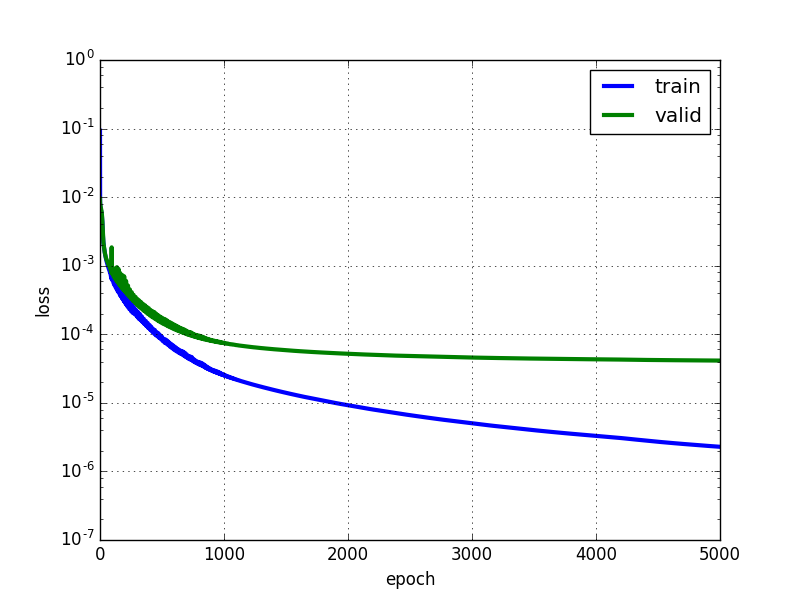
\includegraphics[scale=0.45]{images/loss_model_1}}
	\caption{Learning curves of the first model.}
	\label{figloss1}
\end{figure}~\\
\begin{figure}[h!]
	\centerline{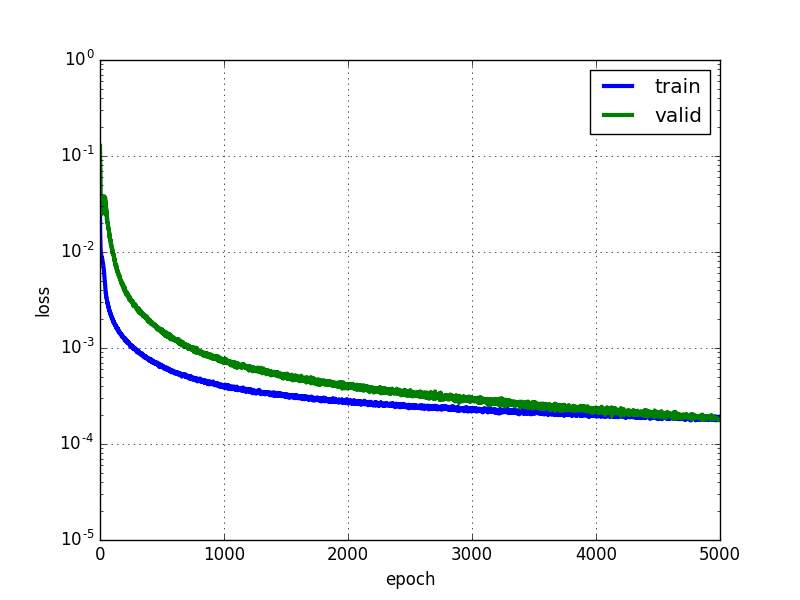
\includegraphics[scale=0.45]{images/loss_v16}}
	\caption{Learning curves of the last model.}
	\label{figloss}
\end{figure}~\\[0.1cm]
Fig.\ref{figloss1} and \ref{figloss} show the training errors and the validation errors of a training time on the first and the third model, respectively. The blue curve presents RMSE on training set, the green curve presents the validation error. Clearly, the overfitting has appeared in the first model. In Fig.\ref{figloss1}, we can see that if the training is able to decrease with the number of epochs\footnote{An epoch is a single pass through the full training set.}, it is not the case of validation loss. At the opposite in the third model, we can see some different values for the two losses at the beginning but after several epochs, these values become more proximate and the overfitting problem has been solved.

Fig.\ref{figrsexample} shows the predicted landmarks on test images set by the thrid model. When we consider the distance between the predicted and manual landmarks, the accuracy on coordinates of predicted landmarks on Fig.\ref{figsub1} is $99\%$. The propotion on Fig.\ref{figsub2} is $80\%$.

\begin{figure}[h]
    \centering
    \begin{subfigure}[t]{0.25\textwidth}
        \centering
        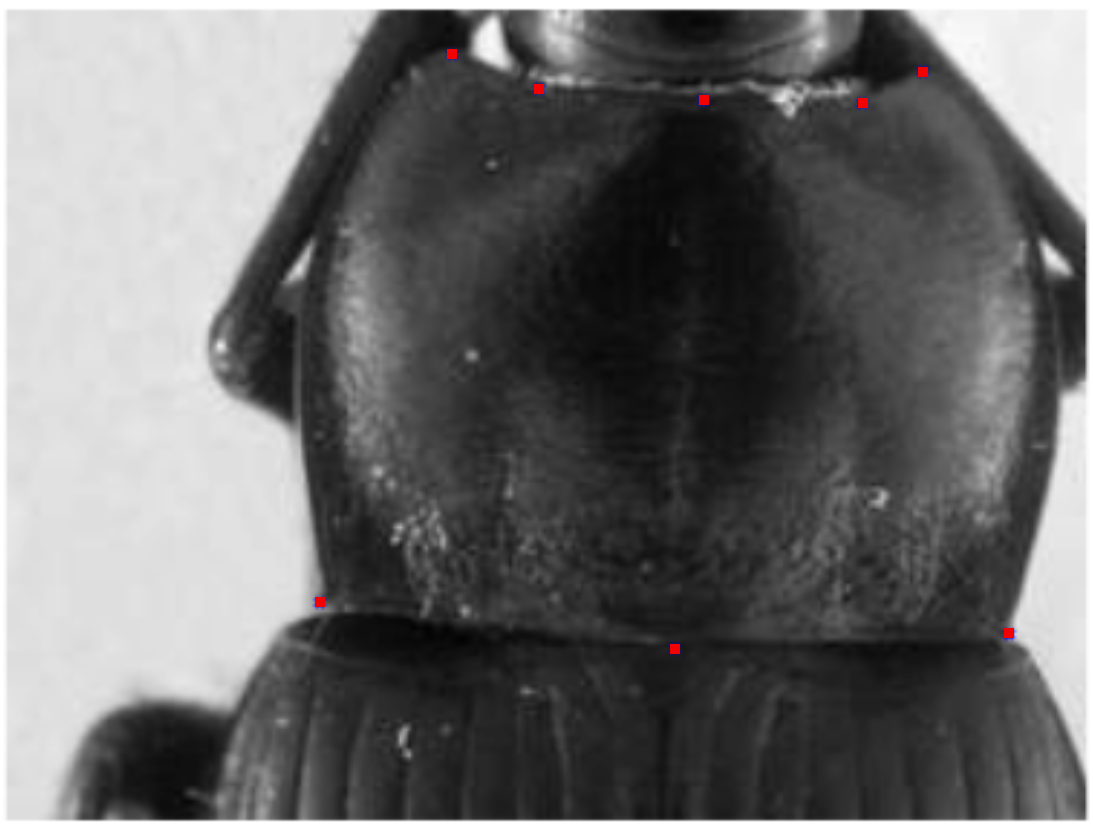
\includegraphics[height=1.2in]{images/plandmark}
        \caption{Image with well-predicted landmarks}
        \label{figsub1}
    \end{subfigure}%
    ~ 
    \begin{subfigure}[t]{0.25\textwidth}
        \centering
        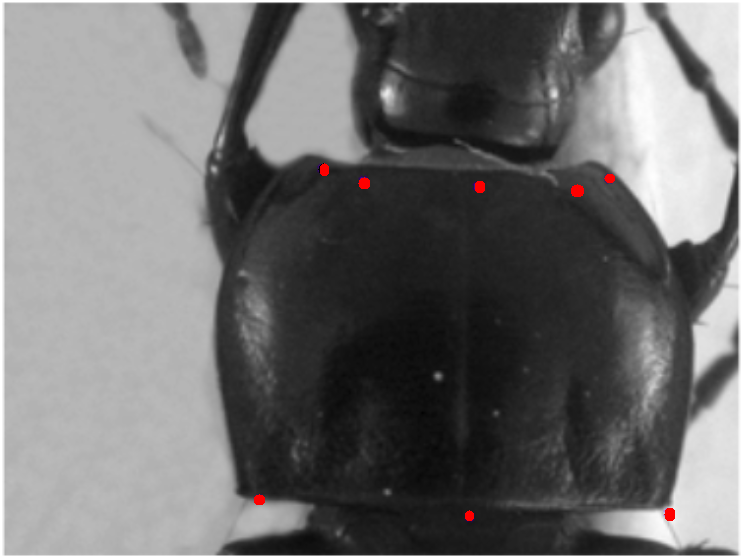
\includegraphics[height=1.2in]{images/plandmark2}
        \caption{Image with inaccuracy landmarks}
        \label{figsub2}
    \end{subfigure}
    \caption{The predicted landmarks on an image in test set (red points)}\
    \label{figrsexample}
\end{figure}
Besides the losses of training, the distance from predicted landmarks to manual landmarks of the test images deserve attention also. Firstly, the distance between them is calculated. Then, the standard deviation \cite{bland1996statistics} is used to quantify the dispersion of a set of distances. Table.\ref{tab2} shows the average error distance given on each landmark.

\begin{table}[htbp]
\caption{The average distance per landmark}
\begin{center}
\begin{tabular}{|c|p{1.5cm}|}
\hline
\textbf{$\#$Landmark} & \textbf{Distance} \\ \hline
1 & 4.002  \\ \hline
2 & 4.4831 \\ \hline
3 & 4.2959 \\ \hline
4 & 4.3865 \\ \hline
5 & 4.2925 \\ \hline
6 & 5.3631 \\ \hline
7 & 4.636 \\ \hline
8 & 4.9363 \\ \hline
\end{tabular}
\label{tab2}
\end{center}
\end{table}

Fig.\ref{figchartlm1} shows the distribution of the distances on the first landmarks of all images. The accuracy based on the distance of each image can be separated into three spaces: the images have the distance less than average value ($4$ pixels): \textbf{56.66$\%$}; the images have the distance from average value to $10$ pixels: \textbf{40.27$\%$}; and the images have the distance greater than $10$ pixels: \textbf{3.07$\%$}. The network has enabled to detect the landmark on pronotum automatically. %If we consider the distance less than average value are good,

\begin{figure}[htbp]
	\centerline{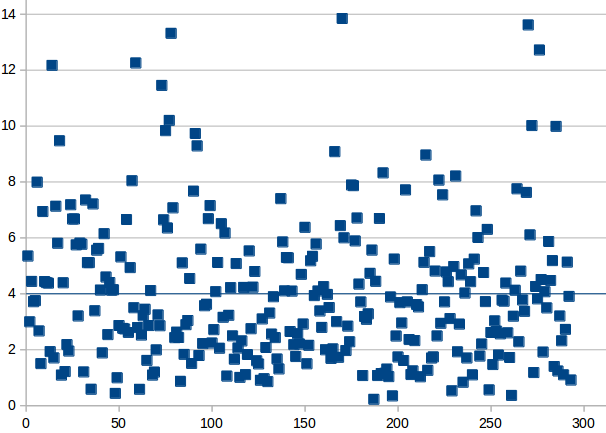
\includegraphics[scale=0.3]{images/statistic}}
	\caption{The distribution of the distances on the first landmark. The blue line is the average value of all distances.}
	\label{figchartlm1}
\end{figure}
Fig.\ref{figchart} shows the proportion of acceptable landmarks. In our case, a predicted landmark is acceptable if the distance between it and corresponding manual landmarks is less than the average distance plus a value of standard deviation. Most of the landmarks have been detected with the accuracy greater than $70\%$. %However, we can see a vast difference between the correlation coefficient results and the proportions on each landmark.

\begin{figure}[htbp]
	\centerline{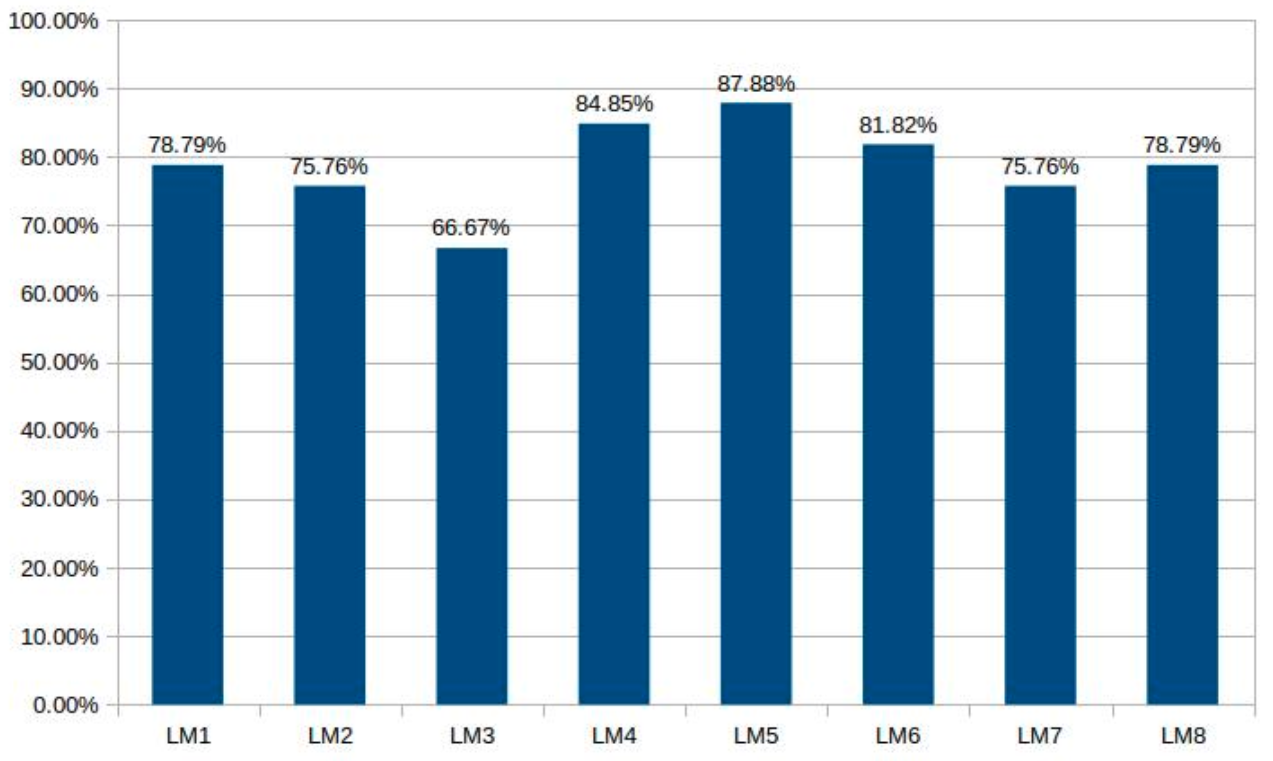
\includegraphics[scale=0.2]{images/chart}}
	\caption{The proportion of acceptable predicted landmarks}
	\label{figchart}
\end{figure}

At the test phase, the trained network is used to predict the landmarks on a set of test images. The program outputs the predicted-landmarks of the images as TPS files; in additional, it also fills and displays the predicted-landmarks on sixteenth firstly images of test data. With the outputs are TPS files, the user can use MAELab \cite{le2017maelab} framework\footnote{MAELab is a free software written in C++. It can be directly
and freely obtained by request at the authors.} to display the landmarks on the images.
\section{Conclusion and future works}
With beetle mandibles images, the object is easy to segment and we have succeeded to determine the landmarks automatically. In opposite, the pronotum images are difficult to segment. Methods which not suppose to be based on segmentation are necessary. In this paper, after testing several models, we have presented a convolutional neural network for automatic detection landmarks on the pronotum. It includes three times repeated structure which consists of a convolutional layer, a max pooling layer, and a dropout layer, followed by the connected layers. During the training phase, suitable techniques are used to prevent overfitting, a common issue of the neural networks. The network was trained several times in different selections of training data. After training with the manual landmarks given by the biologist, the network is able to predict the landmarks on the set of unseen images.

The results from the test set have been evaluated by calculating the distance between manual landmarks and corresponding predicted-landmarks. The average of distance errors on each landmark has been also considered. Using the convolutional network to predict the landmarks on biological images is promising good results in the case that the image can not be segmentation. The quality of prediction allows using automatic landmarking to replace manual landmarks in some aspects.  In our case, the training dataset is limited. As a result, the accuracy of the network is acceptable. However, when we expect more about the accuracy of predicted landmarks (coordinates of predicted landmarks), the result of this work is still needed to improve (for example using a larger training dataset). Therefore, future research in landmarking identification appears as an improved of the worth exploring.

\subsection{Evalution metrics for further predicted landmarks usage}

TODO \\

\section{Discussion}

TODO : a biological part, a computational part \\

\bibliography{includes/references}

\end{document}














In the content of this study, we work on pronotum part of beetle. The provided dataset contains 293 images, each image with 8 landmarks provided by biologists. The dataset was split into a training set with 260 images (training and validation) and a testing set of 33 images. During the training, the network learned the information through a pair of \textit{(image, landmarks)} in training set. At the testing phase, the image without landmarks was given to the trained network and the predicted landmarks will be given at the output. Fig. \ref{figpronotum} shows an example of pronotum image with its manual landmarks.

\begin{figure}[h!]
	\centerline{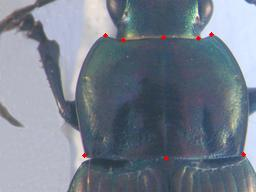
\includegraphics[scale=0.8]{images/pronotum}}
	\caption{An example of pronotum with manual landmarks}
	\label{figpronotum}
\end{figure}

In some succeed networks \cite{krizhevsky2012imagenet}\cite{sun2013deep}\cite{cintas2016automatic}, the maximum size of the inputs is not over 256 pixels. In our case, the resolution of the image is large, it becomes a difficulty for the network. During training and testing, the images are down-sampling to the new resolution of $256 \times 192$. Certainly, the landmark coordinates of the image are also scaled to suit their new resolution. 

The proposed network has a large number of learnable parameters. In addition, the size of the dataset is limited, this means that overfitting will occur during the training process. Therefore, we need to enlarge the size of the dataset. In image processing, we usually apply transform procedure (i.e rotate, translate) to generate a new image but in fact, when we compute the value of the pixels, it does not change while CNN computes the values of the pixels.Therefore, we have applied two other procedures to increase the number of images in the dataset. To address this problem, we have applied two procedures to enlarge the size of the dataset.

The first procedure was applied to change the value of each channel in the original image. According to this, a constant is added to a channel of RGB image and for each time, we just change the value of one of three channels. For example, from an original RGB image, if we add a constant $c = 10$ to the red channel, we will obtain a new image with the values at red channel by greater than the red channel of original image a value of 10. By this way, we can generate three new RGB images from a RGB image.

The second procedure is splitting the channels of RGB images. It means that we separate the channels of RGB into three gray-scale images. This work seems promising because the network works on single-channel images. At the end, we can generate six versions from an image, the total number of images used to train and validate is $260 \times 7 = 1820$ images (six versions and original image). The number of images that used for training and validation is splitted randomly by a ratio (training: $80\%$, validation: $20\%$) that has been set during the network setup.